\begin{frame}{A Lightweight Relu-Based Feature Fusion For Aerial Scene Classification}
    \begin{itemize}
        \item Foco em uma abordagem leve e eficiente
        \item Extração de layers específicos da MobieNetV2
        \begin{itemize}
            \item Entre as camadas de Batch Normalization há ativações ReLU
            \item Busca o maior valor de \(\alpha = \frac{Z_{prev}}{Z_next} \)
            \item Indica o percentual de zeros antes e depois da ativação ReLU
            \item Procura o que tem mais itens por possuir maior representabilidade dos dados
            \item Layers extraidos: 3, 6, 13, 16
        \end{itemize}
        
        \item Global Average Pooling e redução de dimensionalidade por PCA e LDA

        \item Classificação por SVM do tipo one-vs-rest

        \item Acurácia de 93,64\% no AID e 88,05\% no NWPU
    \end{itemize}
\end{frame}

%%%%%%%%%%%%%%%%%%%%%%%%%%%%%%%%%%%%%%%%%

\begin{frame}{Neighbor-Based Label Distribution Learning to Model Label Ambiguity for Aerial Scene Classification}
    \begin{itemize}
        \item \textbf{Ambiguidade em imagens aéreas:}
        \begin{itemize}
            \item Áreas residenciais podem conter estradas.
            \item Elementos visuais similares aparecem em diferentes classes (ex.: zona comercial vs. residencial).
        \end{itemize}
        \item Não utiliza um rótulo único
        \item Gera uma distribuição de rótulos baseado na similaridade visual e na correlação de rótulos entre vizinhos próximos
        \item Testes na VGG16 e na ResNet50
        \item Acurácia de 94,11\% no AID e 89,90\% no NWPU com a ResNet50
    \end{itemize}
\end{frame}

%%%%%%%%%%%%%%%%%%%%%%%%%%%%%%%%%%%%%%%%%

\begin{frame}{Vision Transformers for Remote Sensing Image Classification}
    \begin{itemize}
        \item Utilização de \textit{data augmentation} para gerar mais imagens
        \begin{itemize}
            \item CutOut: Remoção de uma parte aleatória da imagem
            \item MixUp: Sobreposição de uma imagem em cima de outra
            \item CutMix: Recorta partes de uma imagem e adiciona em outra
        \end{itemize}
        \begin{figure}
            \centering
            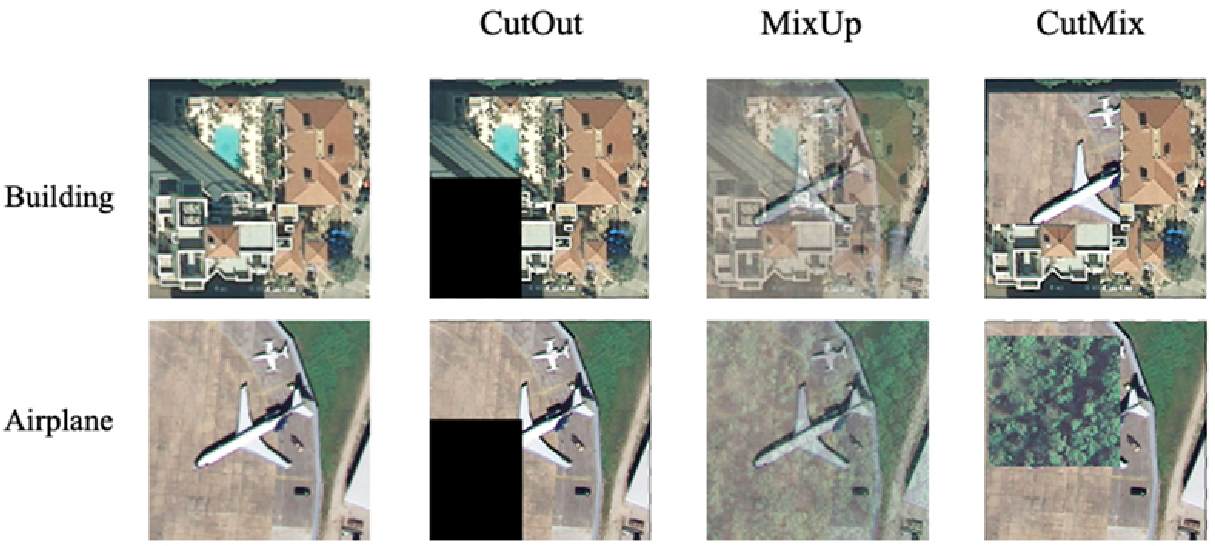
\includegraphics[width=0.75\linewidth]{TrabalhosRelacionados/DataAugmentation.png}
            \caption{Data augmentation}
        \end{figure}
    \end{itemize}
\end{frame}

\begin{frame}{Vision Transformers for Remote Sensing Image Classification}
    \begin{itemize}
        \item Uso de Vision Transformers para a extração de características
        \item Acurácia de 98,48\% no Merced; 95,86\% no AID e 95,56\% no Optimal31
    \end{itemize}
    \begin{figure}
        \centering
        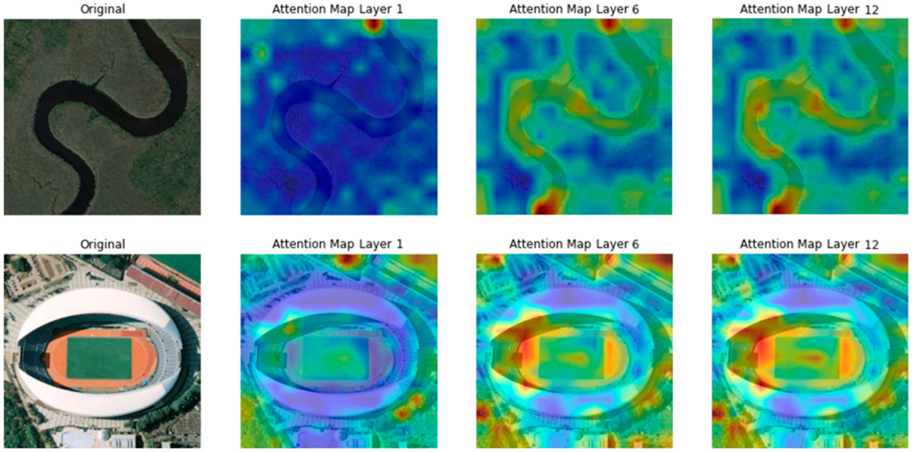
\includegraphics[width=0.75\linewidth]{TrabalhosRelacionados/MapasDeAtençãoAID.png}
        \caption{Mapas de atenção do AID}
        \label{fig:enter-label}
    \end{figure}
    
\end{frame}

%%%%%%%%%%%%%%%%%%%%%%%%%%%%%%%%%%%%%%%%%

\begin{frame}{A Local–Global Interactive Vision Transformer for Aerial Scene Classification}

    \begin{itemize}
        \item Imagens de itens semelhantes podem ter tamanhos diferentes por estarem mais pertos ou mais distantes dos objetos;

        \item ViT com dois patch sizes diferentes, small e large, para extrair diferentes informações da imagem;

        \item Rede totalmente conectada para extrair informações globais.
    \end{itemize}

    \begin{figure}
        \centering
        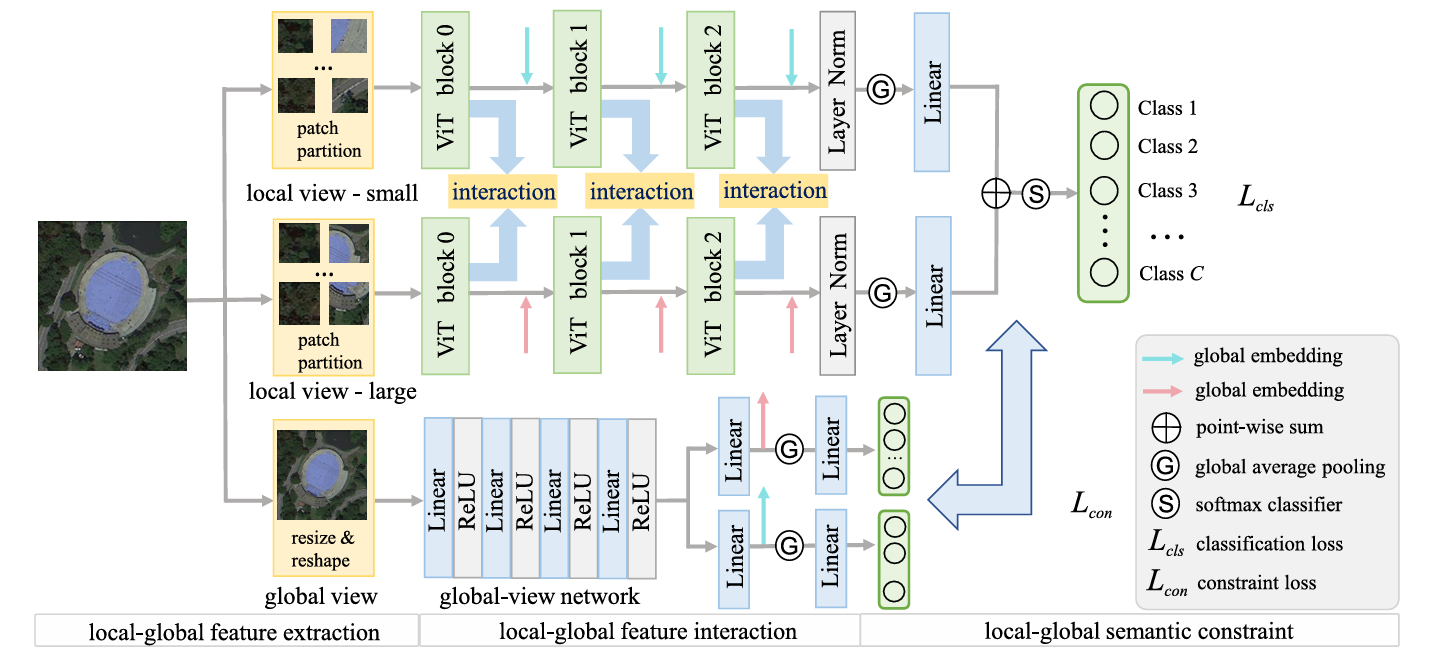
\includegraphics[width=0.5\linewidth]{TrabalhosRelacionados/A_LocalGlobal_Model.png}

    \end{figure}
\end{frame}

\begin{frame}{A Local–Global Interactive Vision Transformer for Aerial Scene Classification}
    \begin{itemize}
        \item Informações agrupadas por um sistema de self-attention

        \item Normalização do softmax para a saída das duas ramificações: \(\hat{p} = softmax(p^{s}+p^{l})\)

        \item \textit{Loss} de \textit{cross-entropy} para garantir a coesão das predições:

        \[L_{\text{cls}} = -\frac{1}{N} \sum_{j=1}^{N} \left( p_j \log \hat{p}_j + (1 - p_j) \log(1 - \hat{p}_j) \right) \]

        \item Acurácia de 99,93\% no UCM, 97,67\% no AID e 95,60\% no NWPU
        
        
    \end{itemize}
\end{frame}

%%%%%%%%%%%%%%%%%%%%%%%%%%%%%%%%%%%%%%%%%

\begin{frame}{When CNNs Meet Vision Transformer: A Joint Framework for Remote Sensing Scene Classification}
    \begin{itemize}
        \item Extração de informações com um Vision Transformer e por CNNs (ResNet34/MobileNetV2)

        \item \textit{Features} extraídas são mescladas para a predição final do modelo

        \begin{figure}
            \centering
            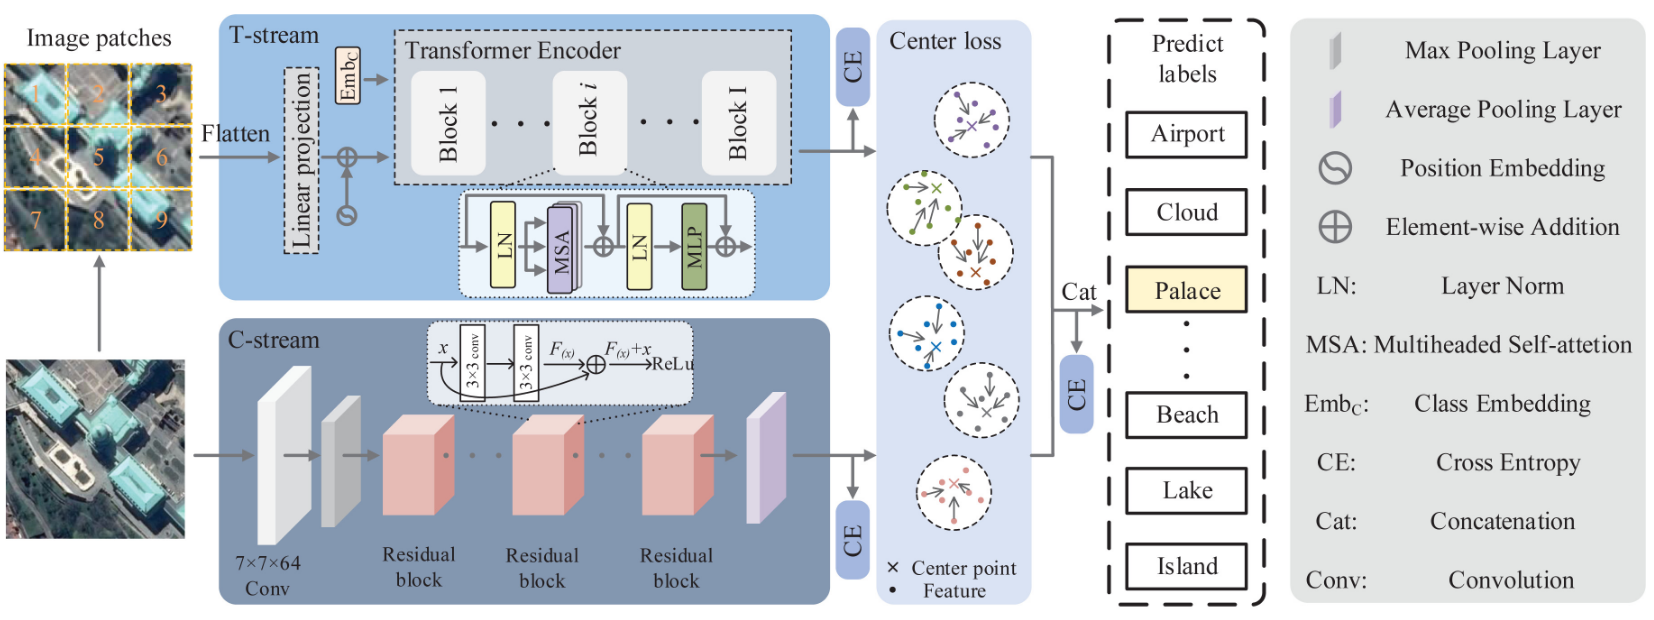
\includegraphics [width=0.75\linewidth]{TrabalhosRelacionados/when_cnns_meet_vision_transformer.png}
        \end{figure}
        
    \end{itemize}
\end{frame}

\begin{frame}{When CNNs Meet Vision Transformer: A Joint Framework for Remote Sensing Scene Classification}
    \begin{itemize}
        \item Feita uma predição para cada ramo

        \item Uso da \textit{Center loss} para garantir a coesão entre as predições dos ramos

        \item Acurácia de 95,49\% no conjunto NWPU e de 97,70\% no conjunto AID.
        
    \end{itemize}
\end{frame}

%%%%%%%%%%%%%%%%%%%%%%%%%%%%%%%%%%%%%%%%%

\begin{frame}{Comparação de resultados}
    \scriptsize % or \footnotesize
    \begin{table}
        \centering
        \begin{tabular}{@{}ccccc@{}}
            \toprule
            \textbf{Artigo} & \textbf{Metodologia} & \textbf{Base de dados} & \textbf{Acurácia} \\ \midrule
            Trabalho 1 & CNN + PCA + LDA + SVM & AID  & 93,64\% \\
                      &                        & NWPU & 88,05\% \\ \midrule
            Trabalho 2 & Redes Convolucionais & AID & 94,11\% \\
                      &                       & NWPU & 89,90\% \\ \midrule
            Trabalho 3 & Vision Transformers & Merced  & 98,48\% \\
                      &                      & AID  & 95,86\% \\
                      &                      & Optimal31 & 95,56\% \\  \midrule
            Trabalho 4 & Vision Transformers + Redes Neurais & UCM  & 99,93\% \\
                      &                                      & AID  & 97,67\% \\
                      &                                      & NWPU & 95,60\% \\  \midrule
            Trabalho 5 & Vision Transformers + CNNs & NWPU & 95,49\% \\
                      &                             & AID & 97,70\% \\ \bottomrule
        \end{tabular}
    \end{table}
\end{frame}
